% Gauss, Werke X/1 (1917), native63–64, printed56–57.
\SourceLeaf{063}\NoSourceHead
\SourceGroup{IX}
\HistoricTitle{HAUPTMOMENTE DES BEWEISES FÜR DIE BIQUADRATISCHEN RESTE.}
\HistoricCitation{[Ein Zettel in Ec3, Kapsel 43.]}
\par\indent Rest $a+bi=m$, Modulus $A+Bi=M$, beide $\equiv1\ (\mathrm{mod.}\ 2+2i)$.

1. Man bildet den ersten Quadranten von $M$ und macht durch Division mit $m$ dessen Variegation.

2. Man verbinde den Punkt $0$ auf irgend eine Weise, doch ohne aus den Ligamenten der Variegation herauszugehen, mit $\dfrac{m-1}{1+i}$ durch die Linie $l$ und zieht gleichfalls die Linien $(l',l'',l''')$
\[
il+m,\ -l+(1+i)m,\ -il+im.
\]
\noindent Dadurch wird das ganze Quadrat, das mittelste Quadrat abgerechnet, welches ohnehin den Intensor $0$ hat, in $4$ Theile symmetrisch getheilt; zwischen $l$ und $l'$ liegt $Q$, zwischen $l'$ und $l''$ liegt $Q'$ u. s. w.
\begin{center}
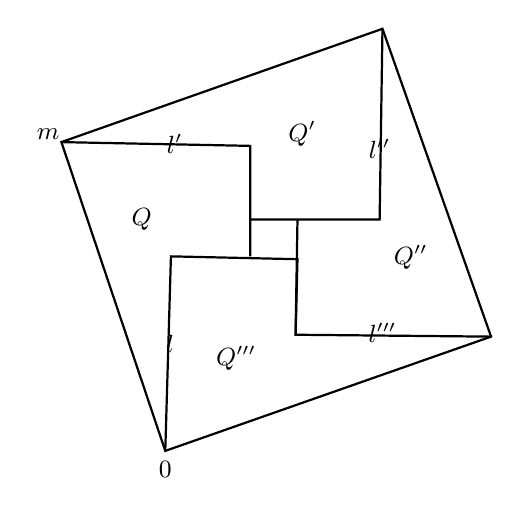
\begin{tikzpicture}[x=.012cm,y=.012cm,line width=.8pt,font=\small]
\draw (0,327)--(340,447)--(455,121)--(110,0)--cycle;
\draw (0,327)--(200,323)--(200,206);
\draw (110,0)--(116,206)--(250,203)--(248,123)--(455,121);
\draw (340,447)--(337,245)--(200,245);
\draw (250,245)--(248,123);
\node at (-14,335) {$m$};\node at (110,-20) {$0$};
\node at (115,113) {$l$};\node at (120,325) {$l'$};
\node at (337,320) {$l''$};\node at (340,125) {$l'''$};
\node at (85,245) {$Q$};\node at (255,336) {$Q'$};
\node at (370,205) {$Q''$};\node at (185,98) {$Q'''$};
\end{tikzpicture}
\end{center}
\clearpage

\SourceLeaf{064}\ArithmeticHead{57}{R}{BIQUADRATISCHE RESTE.}
\par\indent 3. Es sei $-iQ'''=Q^{\mathrm{IV}}$. Wir setzen an die Stelle von $Q'''$ dessen Variegation $Q^{\mathrm{IV}}$; allein, da dessen Quadrate durchgehends Intensoren haben, die um $1$ kleiner sind als die Intensoren von $Q'''$, so wird noch der ganze Inhalt von $Q^{\mathrm{IV}}$ hinzuzusetzen seyn. Der Apparat sieht also so aus:
\begin{center}
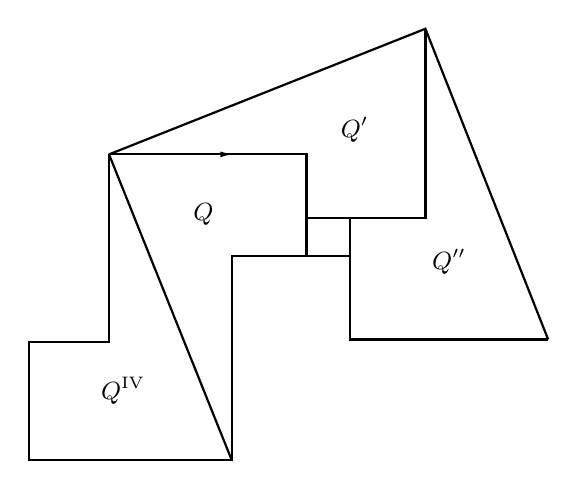
\begin{tikzpicture}[x=.012cm,y=.012cm,line width=.8pt,font=\small]
\draw (0,324)--(335,457)--(465,128);
\draw (0,324)--(130,0);
\draw (0,324)--(0,125)--(-85,125)--(-85,0)--(130,0)--(130,216)--(255,216)--(255,128)--(465,128);
\draw (0,324)--(209,324)--(209,216);
\draw (335,457)--(335,257)--(209,257);
\draw (255,257)--(255,216);
\fill (118,327)--(128,324)--(118,321)--cycle;
\node at (100,260) {$Q$};\node at (260,350) {$Q'$};
\node at (360,210) {$Q''$};\node at (15,74) {$Q^{\mathrm{IV}}$};
\end{tikzpicture}
\end{center}
\par\indent 4. Ebenso sei
\[
Q''-im=Q^{\mathrm{V}},\ im-iQ'=Q^{\mathrm{VI}};
\]
\noindent die Intensoren von $Q^{\mathrm{VI}}$ sind die von $Q$ negativ, genau so wie die von $Q^{\mathrm{V}}$ . . . .
\begin{center}\textbf{BEMERKUNG.}\end{center}
\begingroup\small
\par\indent Vgl. zu diesem Bruchstücke die »\textit{Vorbereitungen zur allgemeinen Theorie der biquadratischen Reste}« Werke II, S. 326—331. Unter »Variegation des ersten Quadranten von $M$ durch Division mit $m$« dürfte das Quadrat mit dem Ecken $0$, $\dfrac M m$, $(1+i)\dfrac M m$, $i\dfrac M m$ zu verstehen sein. Der Begriff des Intensors wird a. a. O. in art. 4, Werke II, S. 328 festgesetzt. Statt »Ligamenten« braucht \textsc{Gauss} daselbst den Ausdruck »Ligaturen«; man geht wohl nicht fehl, wenn man dem Bruchstücke ein früheres Datum beilegt als den »Vorbereitungen«. Dasselbe dürfte gelten für Notizen des Nachlasses im Handbuch 18, Bd (begonnen Oktober 1805) S. 248—256 und andere in der Scheda An, S. 74—88 befindliche Studien, von denen \textsc{Schering} in seiner Fußnote Werke II, S. 334 Gebrauch gemacht zu haben scheint, die sich aber ihrer allzu skizzenhaften Form wegen zur Veröffentlichung nicht eignen.
\begin{flushright}\textsc{Bachmann.}\end{flushright}
\ClosingRule
\vfill\noindent X$_1$.\hfill8\par
\clearpage\endgroup
